\chapter{Current results}\label{r:results}
\section{Diamond}
I investigated diamond crystal. I considered here the case where we have only one set of $s$, $p_z$, $p_y$, and $p_z$ orbitals at each
atomic site.
\begin{figure}[h] 
 \begin{center}
  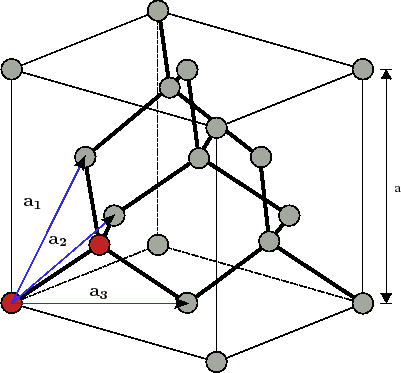
\includegraphics[width=0.3\linewidth]{img/diamond_crystall}
  \caption{Diamond crystall structure.}
 \end{center}
\end{figure}

\begin{table}[h]
 \begin{center}
  \begin{tabular}{|c|c|}
  \hline
    Parameter&Value, [eV]\\ \hline
    $\epsilon_s$ & $0.0$ \\ \hline
    $\epsilon_p$ & $7.4$ \\ \hline
    $V_{\sigma ss}$ & $-3.8$  \\ \hline
    $V_{\sigma sp}$ & $4.44$\\ \hline
    $V_{\sigma pp}$ & $-1.325$ \\ \hline
    $V_{\pi pp}$ &  $4.9$\\ \hline
  \end{tabular}
 \end{center}
  \caption{Interaction parameters for diamond.}
\end{table}

\begin{figure} 
  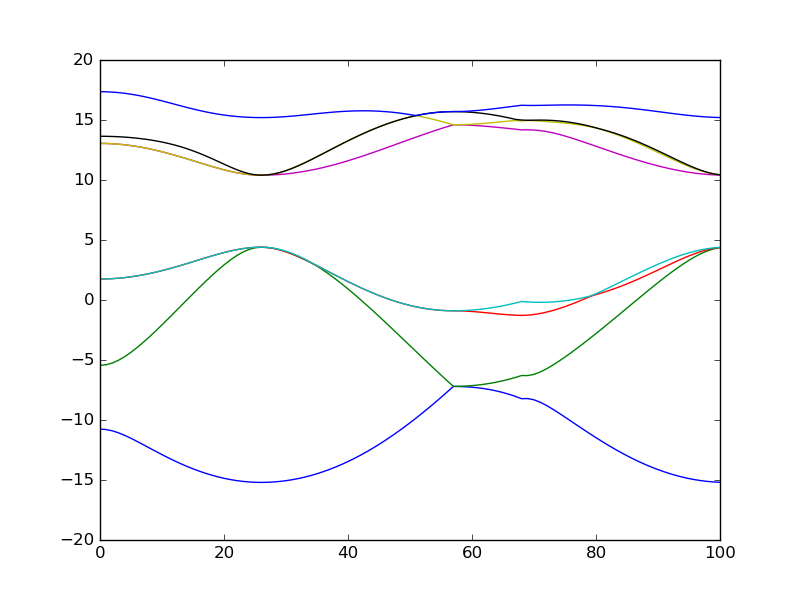
\includegraphics[width=\linewidth]{img/diamond_sp}
  \caption{Calculated band structure of diamond.}
\end{figure}
\begin{figure} 
\begin{center}
  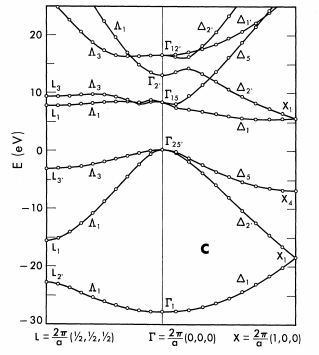
\includegraphics[width=0.5\linewidth]{img/diamond_exp_band_struct}
  \caption{Band structure of diamond (experiment).}
\end{center}
\end{figure}  
